\section{Bracelet}
The bracelet is the part of project that is a cover meant to secure the PCB and be worn by a lifeguard.\\
Short description about the idea behind (to learn more read about the PCB design for the bracelet in electronics chapter):\\
Bracelet is worn by the lifeguard while swimming to the drowning person and on their way back to the shore. The button in the bracelet 
is pressed by the lifeguard, then the coordinates of the lifeguard are sent to the boat.\\
The bracelet should be as small as possible. It cannot handicap the lifefguard during swimming as well as during saving the drowning person.
The recuirements for the project were to design a PCB. The bracelet described in this report is a prototype.\\
The prototype is too big to be used normally. However, it was designed to be as small as possible in respect to the PCB and battery size. 
The bracelet is not main part of the project and is the "nice to have" part of it. If the project would be developed, the PCB would be 
created from smaller components, that are usually more expensive and had to be ordered. Like small SMD components, only a chip of a 
microcontroller, e.g. not the whole Arduino Nano, but only ATmega328p.\\
The design consists of 4 main components:
\begin{itemize}
    \item Top cover.\\
     This is the part printed from TPU. It makes pressing the button from the PCB possible. Also if anyone hits the top
    of the bracelet it makes less harm, than PLA would. The 3D printing is not 100\% waterproof, so the idea would be to cover it by silicon, 
    resin or another waterproofing paint etc.
    \item Bottom cover. \\
    This part had to be done from harder than TPU material, because it has to have the watch bracelet attached to it.
    It makes it not as safe as needed, but because it is a prototype it is acceptable. The 3D printing is not 100\% waterproof, so the idea would be to cover it by silicon, 
    resin or another waterproofing paint etc.
    \item Acrylic rectangle. \\
    This part of the bracelet is supposed to pressure the TPU to the PLA. Since the TPU top cover is not strong/hard enough 
    to be able to make the connection of both top and bottom covers waterproof.
    \item Bracelet. \\
    The bracelet for the hand is taken from a watch found in one of the group members house. The CAD design is adjust in respect to its size.
\end{itemize}
In the first design \autoref{Figure: bracelet first try} the Acryclic rectangle was 3D printed from PLA, but because of the size of it, it was breaking and was not hard enough to 
press the TPU onto the PLA bottom part. Another problem with the first design was that the rectangle was too small, therefore it was decided 
to make the bottom cover wider as well as the rectangle. And that the rectangle should be done from acrylic.\\
\begin{figure}[H]
    \centering
    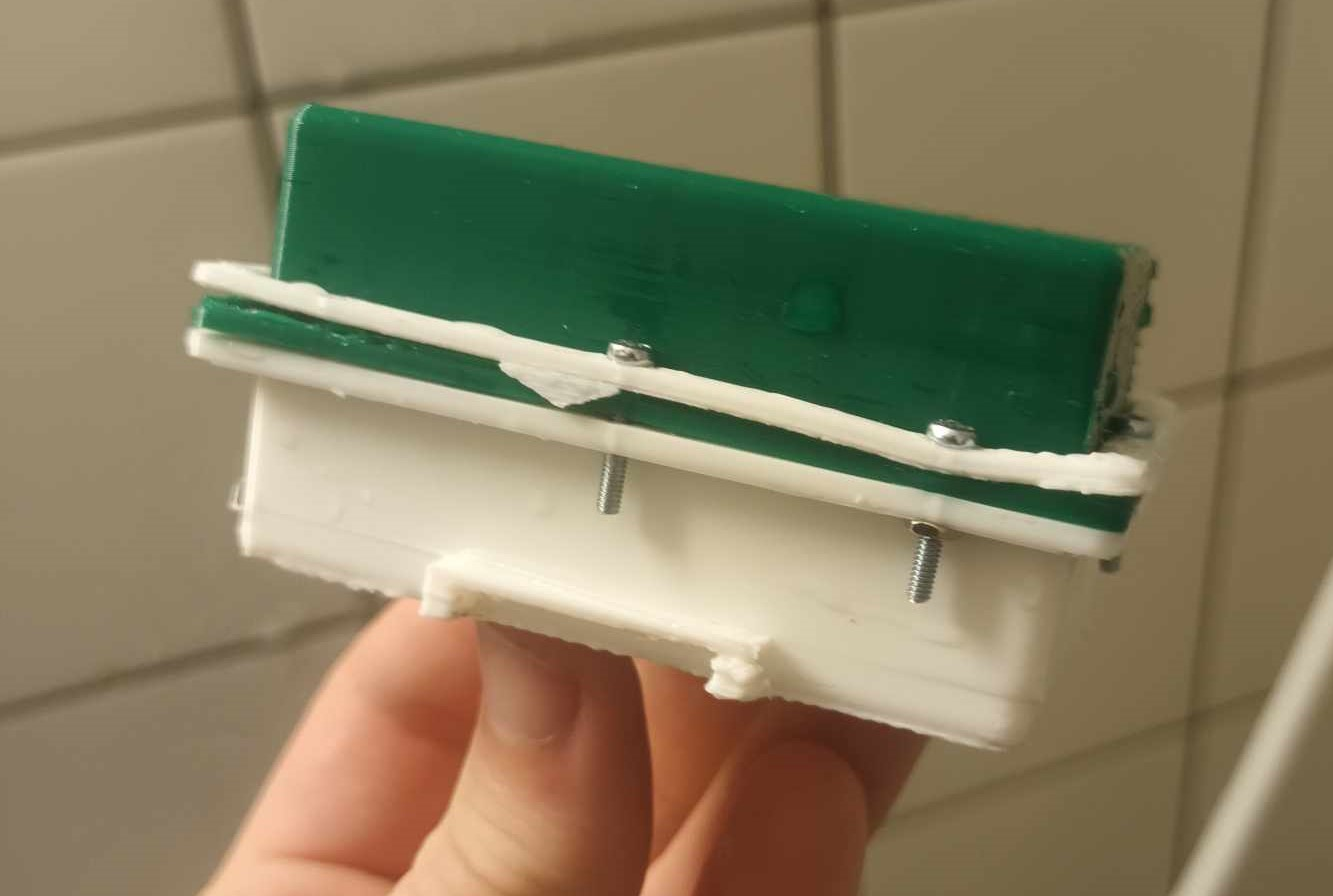
\includegraphics[width=0.7\textwidth]{bracelet_1.jpg}
    \caption{Bracelet First Try}
    \label{Figure: bracelet first try}
\end{figure} 
All in all, the bracelet was not finished due to lack of time. The PCB was done successfully, and the bracelet idea is working as meant to be. 
The design in CAD \autoref{Figure: bracelet CAD design} was done and theoretically would be working. Therefore, it can be said that the bracelet was halfy done.
\begin{figure}[H]
    \centering
    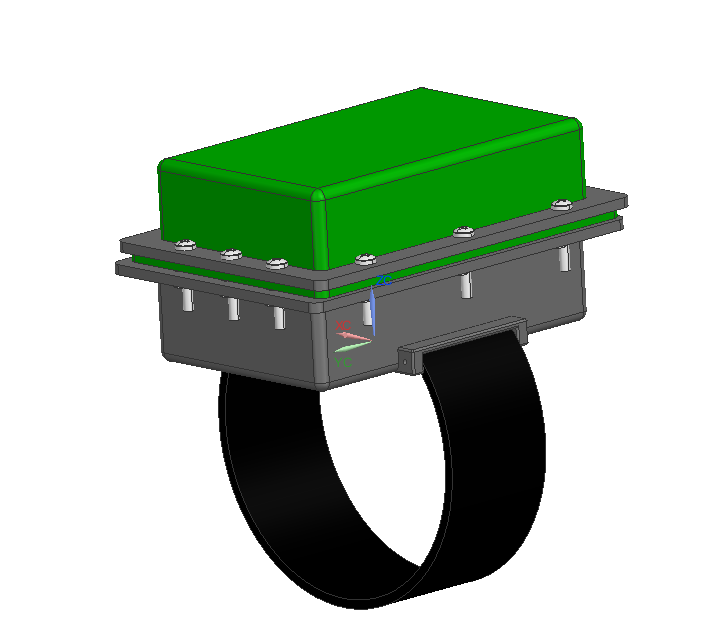
\includegraphics[width=0.7\textwidth]{bracelet.png}
    \caption{Bracelet CAD Design}
    \label{Figure: bracelet CAD design}
\end{figure} 